\chapter{Reference Data and Evaluation Setup}
\label{ch:experiments_setup}

This chapter documents the DNS reference, the LES used for DNS-free sensor placement, sensor data construction, evaluation metrics, baselines, and source availability.

\section{2D Kolmogorov DNS Generation}
\label{sec:dns_generation}

The benchmark is the periodic 2D Kolmogorov flow at $Re=10\,000$, generated in-house to control forcing, viscosity, integration scheme, and snapshot cadence. Configuration, verification, and grid-independence evidence appear in Tables~\ref{tab:dns_params}--\ref{tab:dns_grid_indep}.

\paragraph{Governing equations and characteristic scales.}
On the doubly-periodic square $\Omega = [0, L^\star]^2$, the velocity $\mathbf{u}^\star$~(m/s) and kinematic pressure $p^\star$~(m$^2$/s$^2$) satisfy the incompressible Navier--Stokes equations
\begin{subequations}
\label{eq:ns_dim}
\begin{align}
    \nabla\!\cdot\!\mathbf{u}^\star &= 0, \\
    \partial_{t^\star}\mathbf{u}^\star + (\mathbf{u}^\star\!\cdot\!\nabla)\,\mathbf{u}^\star &= -\nabla p^\star + \nu^\star\,\nabla^2\mathbf{u}^\star + \mathbf{f}^\star,
\end{align}
\end{subequations}
with the Kolmogorov body force $\mathbf{f}^\star = (A^\star \sin(2\pi k_f^\star y^\star),\, 0)^T$. The equations are non-dimensionalised with the box edge $L^\star = 1$~m and a reference velocity $U^\star = 1$~m/s as unit scales; together with $\nu^\star = 10^{-4}$~m$^2$/s this fixes the control Reynolds number $Re \equiv U^\star L^\star/\nu^\star = 10^4$ (equivalently $\nu = 1/Re$ in dimensionless form), prescribed through $\nu^\star$ rather than derived from the realised flow. The physical characteristic scales are the forcing-injection wavelength and the root-mean-square velocity,
\begin{equation}
    \label{eq:char_scales}
    \lambda_f = \frac{1}{k_f} = 0.5~\text{m}, \qquad
    U_{\rm rms} = \sqrt{\langle|\mathbf{u}^\star|^2\rangle} = \sqrt{2\,\overline{\mathrm{KE}}} = 0.503~\text{m/s},
\end{equation}
which set an injection-scale Reynolds number
\begin{equation}
    \label{eq:re_inj}
    Re_f \equiv \frac{U_{\rm rms}\,\lambda_f}{\nu^\star} \approx 2.5\times 10^3 .
\end{equation}
The realised $U_{\rm rms} < U^\star$ because the forced turbulence saturates below the reference velocity, so $Re_f$ is reported as a physical diagnostic while $Re = 10^4$ remains the control parameter set by $\nu^\star$. Table~\ref{tab:dns_params} lists parameters in dimensionless and SI columns. A cross-check at $Re=1\,000$ uses the same protocol with $\nu^\star = 10^{-3}$.

\begin{table}[!htbp]
    \centering
    \caption{DNS configuration at $Re=10\,000$. The SI column uses $L^\star = 1$~m, $U^\star = 1$~m/s, $\nu^\star = 10^{-4}$~m$^2$/s.}
    \label{tab:dns_params}
    \footnotesize
    \setlength{\tabcolsep}{4pt}
    \begin{tabularx}{\textwidth}{
        @{}>{\raggedright\arraybackslash}p{4.4cm}
        >{\raggedright\arraybackslash}X
        >{\raggedright\arraybackslash}X@{}
    }
    \toprule
    \textbf{Parameter} & \textbf{Dimensionless} & \textbf{SI value} \\
    \midrule
    \multicolumn{3}{@{}l}{\emph{Governing equation}} \\
    Equation                  & \multicolumn{2}{@{}l@{}}{Incompressible Navier--Stokes,~\eqref{eq:ns_main}} \\
    Forcing form $\mathbf{f}$  & \multicolumn{2}{@{}l@{}}{Kolmogorov body force,~\eqref{eq:forcing}} \\
    Domain $\Omega$           & $[0,1]^2$, periodic & $[0,1]^2$ m$^2$ \\
    Reynolds number $Re$      & $10\,000$ & $10\,000$ \\
    Kinematic viscosity $\nu$ & $10^{-4}$ & $10^{-4}$ m$^2$/s \\
    Forcing wavenumber $k_f$  & $2$ & $2$ m$^{-1}$ \\
    Forcing amplitude $A$     & $0.1$ & $0.1$ m/s$^2$ \\
    \midrule
    \multicolumn{3}{@{}l}{\emph{Solver method}} \\
    Spatial discretisation       & \multicolumn{2}{@{}l@{}}{Spectral pseudo-spectral, $2/3$-rule dealiasing~\cite{Orszag1971,Boyd2001}} \\
    Time integrator              & \multicolumn{2}{@{}l@{}}{ETDRK4 (exp.\ time differencing)~\cite{Cox2002,KassamTrefethen2005}} \\
    Precision                    & \multicolumn{2}{@{}l@{}}{fp64} \\
    Initial condition            & \multicolumn{2}{@{}l@{}}{Random Gaussian field; spectral burn-in} \\
    \midrule
    \multicolumn{3}{@{}l}{\emph{Discretisation parameters}} \\
    Run resolution $N_{\rm run}$    & $1024 \times 1024$ & $1024 \times 1024$ \\
    Stored resolution $N$           & $256 \times 256$ & $256 \times 256$ \\
    Time step $\Delta t_{\rm DNS}$  & $2.5\times 10^{-4}$ & $0.25$ ms \\
    Time horizon $T$                & $5.0$ & $5.0$ s \\
    Sample interval                 & $0.025$ & $25$ ms \\
    Frames stored                   & \multicolumn{2}{@{}l@{}}{$N_{\rm frames} = 201$ (downsampled $\times 4$ from $N_{\rm run}$)} \\
    \bottomrule
    \end{tabularx}
\end{table}

\paragraph{Solver and storage.}
The solver runs on $N_{\rm run}=1024^2$ with $\Delta t_{\rm DNS}=2.5\times 10^{-4}$, downsampled $4\times$ to $N_{\rm stored}=256^2$ snapshots every $\Delta t_{\rm store}=0.025$~s ($201$ frames over $T=5$); sensor measurements and offline evaluation use this $256^2$ trajectory. \emph{The full trajectory never enters training}; only (a) sensor extraction and (b) offline a posteriori evaluation are permitted.

\paragraph{DNS verification.}
\label{subsec:dns_verification}
Table~\ref{tab:dns_verification} reports verification across three criterion groups on both the $N_{\rm run}=1024^2$ run grid and the $N_{\rm stored}=256^2$ trajectory; statistical diagnostics discard a $20\%$ burn-in. All thresholds pass except $T/t_{\rm eddy}=2.51$, which falls below the long-window ideal; the reconstruction target is therefore treated as a single DNS trajectory rather than a statistically converged ensemble, and the flow statistics reported here are single-trajectory diagnostics (the multi-seed training runs quantify optimisation stochasticity, not flow-statistical convergence).

\begin{table}[!htbp]
    \centering
    \caption{DNS verification at $Re=10\,000$, $T=5$ ($20\%$ burn-in discarded). Derived turbulence scales: $\varepsilon = \nu\langle\omega^2\rangle = 6.27\times 10^{-3}$~m$^2$/s$^3$, $\eta = (\nu^3/\varepsilon)^{1/4} = 3.55\times 10^{-3}$~m, $U_{\rm rms} = \sqrt{2\langle\text{KE}\rangle} = 0.503$~m/s, $t_{\rm eddy} = L^\star/U_{\rm rms} = 1.99$~s.}
    \label{tab:dns_verification}
    \footnotesize
    \setlength{\tabcolsep}{5pt}
    \begin{tabularx}{\textwidth}{
        @{}>{\raggedright\arraybackslash}X
        >{\centering\arraybackslash}p{3.0cm}
        >{\centering\arraybackslash}p{1.8cm}
        >{\raggedright\arraybackslash}p{3.8cm}@{}
    }
    \toprule
    \textbf{Criterion} & \textbf{Threshold} & \textbf{Measured} & \textbf{Verdict} \\
    \midrule
    \multicolumn{4}{@{}l}{\emph{Spatial resolution}} \\
    Pope-2000 on $N_{\rm run}=1024^2$       & $k_{\max}\eta \ge 1.5$ & $7.61$    & $\checkmark$ over-resolved \\
    Pope-2000 on $N_{\rm stored}=256^2$     & $k_{\max}\eta \ge 1.5$ & $1.91$    & $\checkmark$ Pope-resolved \\
    Spectrum tail slope ($k>k_f$, $R^2{=}0.99$) & dissipation-dominated & $-4.61$ & $\checkmark$ consistent \\
    \midrule
    \multicolumn{4}{@{}l}{\emph{Time-step adequacy and numerical stability}} \\
    Advective Courant $U_{\rm rms}\Delta t/\Delta x$ & $\le 0.5$            & $0.13$    & $\checkmark$ \\
    Diffusive $\nu\Delta t/\Delta x^2$         & absorbed by ETDRK4   & $26$      & $\checkmark$ stable under ETD \\
    Solver $\Vert\nabla\!\cdot\!\mathbf{u}\Vert_\infty$ & fp64 round-off   & $\lesssim 10^{-12}$ & $\checkmark$ \\
    Dealiased tail $E(k_f)/E(k_{\max}^{\rm run})$ & $> 10^6$              & $> 10^6$  & $\checkmark$ no pile-up \\
    \midrule
    \multicolumn{4}{@{}l}{\emph{Statistical window}} \\
    Turnover coverage $T/t_{\rm eddy}$       & $\ge 50$ ideal       & $2.51$    & limited; multi-seed used \\
    \bottomrule
    \end{tabularx}
\end{table}

\paragraph{Evaluator constants and stationarity.}
Three DNS-derived constants enter the evaluator of \S\ref{sec:eval_metrics} and Appendix~\ref{app:pressure_limit}: the relative-divergence denominator $\Vert\nabla\mathbf{u}\Vert_F^{\rm DNS} = 8.898$~s$^{-1}$ (FD on $128^2$), the FD evaluator floor $\Vert\nabla\!\cdot\!\mathbf{u}\Vert_2 / \Vert\nabla\mathbf{u}\Vert_F^{\rm DNS} = 1.04\%$, and the gauge-removed pressure $p_{\rm rms} = 0.242$~m$^2$/s$^2$. Three indicators support the short $T/t_{\rm eddy}=2.51$ window: cumulative $\bar{\mathrm{KE}}(T)$ change $<3\%$ over the last $10$ snapshots; dissipation-tail slope variation $\le \pm 0.3$ across $t\in[1,3]$, $[2,4]$, $[3,5]$; and $\langle\mathbf{f}\!\cdot\!\mathbf{u}\rangle$ matching $\nu\langle\omega^2\rangle$ within $5\%$. The tail slope $-4.61$ is steeper than the Kraichnan $k^{-3}$ enstrophy cascade~\cite{Kraichnan1967} because the $[0,1]^2$ box admits no extended inertial range at this $Re$.

\paragraph{Grid independence.}
\label{subsec:dns_grid_indep}
A refinement sweep on $N \in \{128, 256, 512, 1024\}$ at production solver settings ($\Delta t = 2.5\times 10^{-4}$, ETDRK4, $2/3$-rule, fp64) is reported in Table~\ref{tab:dns_grid_indep} and Figures~\ref{fig:grid_indep_convergence}--\ref{fig:grid_indep_main}. The four runs share a deterministic spectral-seeded IC bit-exact at common grid points across $N$, isolating discretisation error from IC variability~\cite{Pope2000}. At production resolution $N=256$, post-spin-up ($t \ge 2$) agreement against $N=1024$ is $0.064\%$ for KE and $0.24\%$ for enstrophy, with $0.05\%$ in the $K=100$ sensor band $k \le k_{\max}^{\rm sensor} \approx 5.64$ (carrying $\approx 99\%$ of the kinetic energy at $t=5$). The $N=512$ row provides ref-converged evidence near fp64 round-off ($\approx 4\times 10^{-7}$). The under-resolved $N=128$ drifts by $7.33\%$ (KE) and $8.76\%$ (enstrophy), confirming the protocol detects insufficient resolution. Consecutive convergence ratios ($115\times$ for $N{=}128{\to}256$, $1.65\times 10^5$ for $N{=}256{\to}512$) far exceed the algebraic $r^p = 4$ baseline, placing the sequence in the pseudo-spectral super-algebraic regime~\cite{Boyd2001}.

\begin{table}[!htbp]
    \centering
    \caption{Grid-independence verification at $Re=10\,000$, $T=5$, against the $N=1024$ reference. Post-spin-up metrics use $t \in [2, 5]$; pointwise $\|\Delta u\|_2 / \|u\|_2$ is reported at $t=0.5$. The ``Ratio vs prev $N$'' column is the ratio of $\Delta$KE between successive grid pairs ($r^p = 4$ algebraic baseline). $\eta = (\nu^3/\varepsilon)^{1/4}$ with $\varepsilon = 2\nu\langle\omega^2\rangle_{N=1024}$ ($k_\eta = 41.5$~m$^{-1}$).}
    \label{tab:dns_grid_indep}
    \footnotesize
    \setlength{\tabcolsep}{4pt}
    \begin{tabularx}{\textwidth}{
        @{}>{\raggedright\arraybackslash}p{1.4cm}
        >{\centering\arraybackslash}p{1.5cm}
        >{\centering\arraybackslash}p{1.9cm}
        >{\centering\arraybackslash}p{1.9cm}
        >{\centering\arraybackslash}p{2.1cm}
        >{\centering\arraybackslash}p{1.8cm}
        >{\centering\arraybackslash}p{1.8cm}@{}
    }
    \toprule
    \textbf{Grid} & \textbf{$k_{\max}/k_\eta$} & \textbf{$\Delta$KE (post-spin-up)} & \textbf{$\Delta$Enstrophy (post-spin-up)} & \textbf{$\Delta E(k\le k_{\max}^{\rm sensor})$} & \textbf{$\|\Delta u\|_2 / \|u\|_2$ at $t=0.5$} & \textbf{Ratio vs prev $N$} \\
    \midrule
    $N=128$  & $1.03$ & $7.33\%$        & $8.76\%$        & $7.26\%$        & $2.60\%$         & -- \\
    $\mathbf{N=256}$  & $2.06$ & $\mathbf{0.064\%}$ & $\mathbf{0.24\%}$  & $\mathbf{0.05\%}$  & $\mathbf{0.113\%}$ & $\mathbf{115\times}$ \\
    $N=512$  & $4.12$ & $3.87\times 10^{-7}$ & $3.78\times 10^{-7}$ & $3\times 10^{-5}\%$ & $5\times 10^{-6}$ & $1.65\times 10^{5}$ \\
    $N=1024$ & $8.23$ & \emph{reference} & \emph{reference} & \emph{reference} & \emph{reference} & -- \\
    \bottomrule
    \end{tabularx}
\end{table}

\begin{figure}[!htbp]
    \centering
    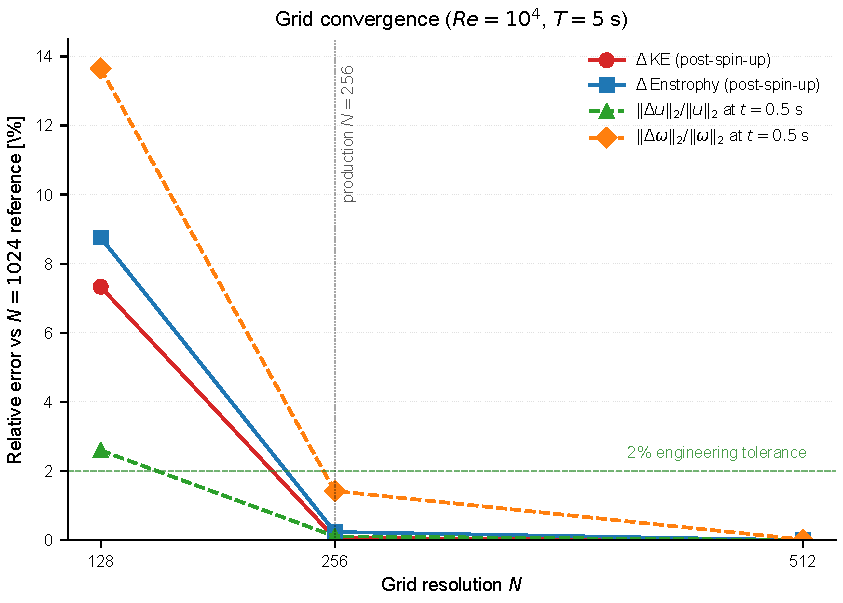
\includegraphics[width=0.72\textwidth]{figures/results/grid_indep_convergence.pdf}
    \caption{Relative error vs.\ grid resolution $N$ ($Re=10^4$, $T=5$~s) against the $N=1024$ reference. Lines: post-spin-up ($t \in [2,5]$~s) maximum relative differences of kinetic energy (KE, m$^2$/s$^2$) and enstrophy (1/s$^2$), and pointwise $L^2$ relative errors of $u$ and $\omega$ at $t=0.5$~s. Horizontal dashed line: $2\%$ tolerance; vertical dashed line: production resolution $N=256$. Values in Table~\ref{tab:dns_grid_indep}.}
    \label{fig:grid_indep_convergence}
\end{figure}

\begin{figure}[!htbp]
    \centering
    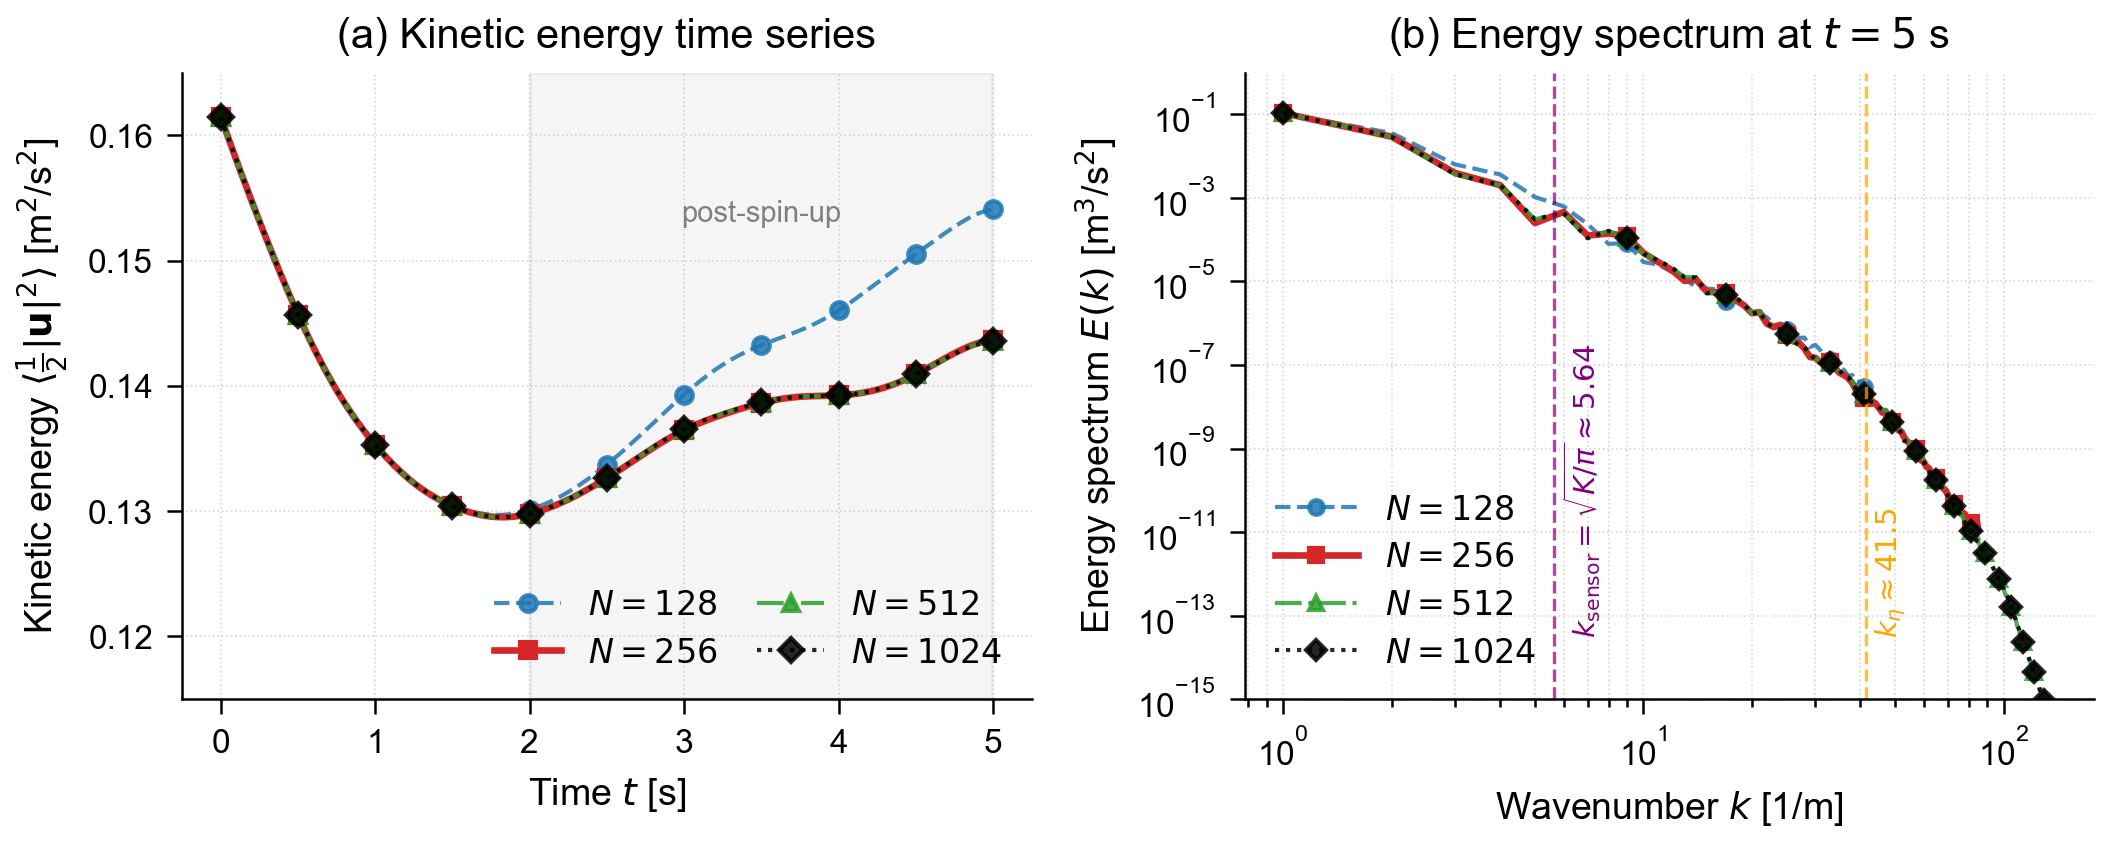
\includegraphics[width=\textwidth]{figures/results/grid_indep_main.png}
    \caption{Grid-independence supporting evidence. (a) Kinetic energy (m$^2$/s$^2$) vs.\ time $t$ (s) for $N \in \{128, 256, 512, 1024\}$; shaded band: post-spin-up window $t \in [2, 5]$~s. (b) Radial energy spectrum $E(k)$ (m$^3$/s$^2$) at $t=5$~s; vertical dashed lines: $K=100$ sensor Nyquist $k_{\rm sensor} = \sqrt{K/\pi} \approx 5.64$~m$^{-1}$ (purple) and dissipation wavenumber $k_\eta = 41.5$~m$^{-1}$ (orange).}
    \label{fig:grid_indep_main}
\end{figure}

\paragraph{Time-step, seed, and IC sensitivity.}
Three supplementary checks isolate non-spatial sources of error. Halving the time step at $N=256$, $T=0.5$ changes the solution by $7.0\times 10^{-6}$ ($160\times$ below the spatial error), confirming $\Delta t = 2.5\times 10^{-4}$ is temporally converged. A second seed reproduces the result: $N=256$-vs-$N=512$ post-spin-up KE agreement is $0.19\%$, within the $2\%$ engineering tolerance. Spectral truncation error is a property of discretisation rather than IC phase~\cite{Boyd2001}, and the $\approx 99\%$ sensor-band energy fraction holds for any forced-stationary trajectory at this $Re$, so the conclusions transfer to the production IC. Per-field log-log convergence and diagnostics across all four grids appear in Appendix~\ref{app:dns_grid_indep_supp}.

\section{LES for DNS-Free Sensor Placement}
\label{sec:les_placement}

In the LES-derived placement strategy (one of the placement options studied), a low-cost LES on a new scene supplies a POD basis from which QR-pivoting selects sensor positions; the physical flow then provides the sensor values. The DNS substitutes for the physical flow during controlled validation, but not for placement. The LES need not match the DNS pointwise: its sole role is to supply a POD snapshot matrix whose leading modes determine the QR-pivot indices. The LES and the DNS are therefore \emph{independent} realisations: they share the same $Re$, domain, and forcing but start from different random initial fields, so at high Reynolds number their trajectories decorrelate and never coincide pointwise at any matched time. Their integration horizons follow their roles, not each other. The LES is integrated long only so that its leading POD modes reach statistical convergence for placement (it is a statistical tool, not a trajectory to be matched); the DNS is the single target realisation to be reconstructed over the shorter window $t\in[0,5]$, from which the sensors read their values. Statistics therefore set the LES horizon and the reconstruction target sets the DNS horizon (the specific values appear in Tables~\ref{tab:dns_params} and~\ref{tab:les_params}).

\paragraph{Filtered equations and closure.}
The LES solves the spatially filtered incompressible Navier--Stokes equations,
\begin{subequations}
\label{eq:filtered_ns}
\begin{align}
    \nabla\!\cdot\!\bar{\mathbf{u}} &= 0, \label{eq:filtered_cont}\\
    \partial_t \bar{u}_i + \bar{u}_j\,\partial_j \bar{u}_i &= -\partial_i \bar{p} + \nu\,\nabla^2 \bar{u}_i - \partial_j \tau_{ij}^{\mathrm{SGS}} + f_i, \label{eq:filtered_mom}
\end{align}
\end{subequations}
on the same domain, viscosity, and forcing as the DNS. The high-wavenumber SGS drain is a spectral hyperviscosity term, used alone in the reference LES; the low-fidelity variant additionally applies a Bardina scale-similarity term~\cite{Bardina1980, Sagaut2006},
\begin{equation}
    \label{eq:bardina_hyperv}
    \begin{aligned}
    \mathcal{D}_{\rm hyper}(\bar{\mathbf{u}}) &= -\nu_h\,(-\nabla^2)^{p}\bar{\mathbf{u}}\quad(p=2), \\
    \tau_{ij}^{\mathrm{Bardina}} &= C_B (\widetilde{\bar{u}_i\,\bar{u}_j} - \widetilde{\bar{u}_i}\widetilde{\bar{u}_j})\quad(C_B = 1.0,\ \text{low-fidelity only}),
    \end{aligned}
\end{equation}
both chosen over Smagorinsky-type eddy-viscosity, which is poorly justified for 2D turbulence with a forced inverse cascade. The solver shares the DNS spatial discretisation (pseudo-spectral, $2/3$-rule dealiasing, fp64) but advances in time with an explicit second-order Runge--Kutta (RK2) scheme rather than the DNS's ETDRK4, with a conservatively small step ($\Delta t = 10^{-4}$~s, below the explicit hyperviscosity stability limit). It differs from the DNS in SGS closure, grid resolution, and time integrator. Reference and low-fidelity discretisation parameters are listed in Table~\ref{tab:les_params}.

\begin{table}[!htbp]
    \centering
    \caption{LES configuration at $Re=10\,000$. The sub-grid closure and the four discretisation parameters at the bottom differ between the reference and low-fidelity runs; values in brackets denote the low-fidelity setting. The governing equation and solver inherit the dimensional mapping of Table~\ref{tab:dns_params}.}
    \label{tab:les_params}
    \footnotesize
    \setlength{\tabcolsep}{5pt}
    \begin{tabularx}{\textwidth}{
        @{}>{\raggedright\arraybackslash}p{5.6cm}
        >{\raggedright\arraybackslash}X@{}
    }
    \toprule
    \textbf{Item} & \textbf{Setting (reference; [low-fidelity])} \\
    \midrule
    \multicolumn{2}{@{}l}{\emph{Governing equation}} \\
    Equation                   & Filtered NS,~\eqref{eq:filtered_ns}; $Re = 10\,000$, $\nu = 10^{-4}$~m$^2$/s \\
    Domain, forcing            & $[0,1]^2$~m$^2$, periodic; $\mathbf{f} = (A\sin 2\pi k_f y, 0)^T$ with $A=0.1$~m/s$^2$, $k_f=2$~m$^{-1}$ \\
    \midrule
    \multicolumn{2}{@{}l}{\emph{Sub-grid closure}} \\
    Form                       & hyperviscosity~\eqref{eq:bardina_hyperv}; $+$ Bardina scale-similarity~[low-fidelity] \\
    Coefficients               & hyperviscosity order $p = 2$; Bardina $C_B = 1.0$ (low-fidelity) \\
    Hyperviscosity tuning $\nu_h$ & per-run drain for a $> 10^6$ dissipation tail between $k_f$ and $k_{\max}^{\rm LES}$ \\
    \midrule
    \multicolumn{2}{@{}l}{\emph{Solver method}} \\
    Spatial / time / precision & spectral, $2/3$-rule dealiasing; explicit RK2 (Heun), $\Delta t = 10^{-4}$~s; fp64 \\
    Initial condition          & random Gaussian field + forced spin-up \\
    \midrule
    \multicolumn{2}{@{}l}{\emph{Discretisation (reference~/~[low-fidelity])}} \\
    Grid resolution $N_{\rm LES}$        & $256^2$~/~$[128^2]$ \\
    Effective $k_{\max}^{\rm LES}$       & $85.3$~m$^{-1}$~/~$[42.7$~m$^{-1}]$ \\
    Time horizon $T_{\rm end}$           & $50$~s ($26.5\,t_{\rm eddy}$)~/~$[15$~s, $7.5\,t_{\rm eddy}]$ \\
    Compute cost                         & $1\times$~/~$[1/16\times]$ \\
    \bottomrule
    \end{tabularx}
\end{table}

\paragraph{Verification.}
\label{subsec:les_verification}
Table~\ref{tab:les_verification} reports verification against three criterion groups. Spatial resolution targets resolved-band spectral overlap with DNS (within $2\times$ on $k\in[2, N_{\rm LES}/3]$) instead of the Pope-2000 criterion, since the SGS closure absorbs the unresolved stress; time-step stability uses a fixed $\Delta t = 10^{-4}$~s held below the explicit hyperviscosity limit (advective Courant $0.007$); statistical convergence is comfortable at $T_{\rm end}/t_{\rm eddy}=26.5$, with $\bar{\mathrm{KE}}(T)$ plateau within $5\%$ over the last $10$ snapshots, sub-window slope stationarity within $\pm 0.4$ slope units, and $\approx 17$ statistically independent POD samples (above the $\sim 10$-sample leading-mode threshold).

\begin{table}[!htbp]
    \centering
    \caption{LES verification for the reference LES ($N_{\rm LES}=256^2$, $T_{\rm end}=50$~s).}
    \label{tab:les_verification}
    \footnotesize
    \setlength{\tabcolsep}{5pt}
    \begin{tabularx}{\textwidth}{
        @{}>{\raggedright\arraybackslash}X
        >{\centering\arraybackslash}p{3.2cm}
        >{\centering\arraybackslash}p{1.8cm}
        >{\raggedright\arraybackslash}p{3.4cm}@{}
    }
    \toprule
    \textbf{Criterion} & \textbf{Threshold} & \textbf{Measured} & \textbf{Verdict} \\
    \midrule
    \multicolumn{4}{@{}l}{\emph{Spatial resolution}} \\
    Spectral overlap with DNS on $k\in[2, N_{\rm LES}/3]$ & within $2\times$       & within $2\times$ & $\checkmark$ leading modes aligned \\
    Pile-up at $k\to N_{\rm LES}/3$                       & none                   & none             & $\checkmark$ dealiasing intact \\
    \midrule
    \multicolumn{4}{@{}l}{\emph{Time-step adequacy and stability}} \\
    Advective Courant $U_{\rm rms}\Delta t/\Delta x$       & $\le 0.5$              & $0.007$          & $\checkmark$ \\
    Hyperviscous stability $\nu_h k_{\max}^{2p}\Delta t$   & $< 1$ (explicit RK2)   & $5\times 10^{-3}$ & $\checkmark$ \\
    Incompressibility $\Vert\nabla\!\cdot\!\bar{\mathbf{u}}\Vert_\infty$ & spectral round-off & $<10^{-10}$ & $\checkmark$ \\
    \midrule
    \multicolumn{4}{@{}l}{\emph{Statistical window}} \\
    Turnover coverage $T_{\rm end}/t_{\rm eddy}$          & $\ge 5$ for POD       & $26.5$           & $\checkmark$ $\gg 5$ \\
    Independent samples $T_{\rm end}/t_{\rm int}$         & $\ge 10$              & $\approx 17$     & $\checkmark$ POD-converged \\
    KE plateau over last $10$ snapshots                   & rel.\ change $<5\%$   & $<5\%$           & $\checkmark$ spin-up cleared \\
    \bottomrule
    \end{tabularx}
\end{table}

\paragraph{Predictability horizon.}
A same-initial-condition diagnostic bounds how long any reference-grade LES can match the DNS pointwise, substantiating the decorrelation premise stated above. The vorticity fields are co-located through $\approx 1\,t_{\rm eddy}$ and visibly separated by $\approx 2\,t_{\rm eddy}$ (Fig.~\ref{fig:les_vort_compare}). The reference LES, initialised from the DNS field at $t=0$ and integrated to $t=5$~s on the matched grid (shared $Re$, domain, and forcing), keeps its velocity relative-$L^2$ error against the DNS below $5\%$ for $0.59\,t_{\rm eddy}$ and below $20\%$ for $1.10\,t_{\rm eddy}$; beyond that, chaotic divergence and the closure difference dominate, and the full-field error peaks near $92\%$ (below the $\sqrt{2}$ fully-decorrelated level) by $t\approx 4$~s (Fig.~\ref{fig:les_predictability}). The energy-containing scales persist longest: the resolved-band ($k\le 5$) error follows the full-field error, and the velocity correlation stays above $0.9$ until $\approx 1.5\,t_{\rm eddy}$, while the small-scale vorticity correlation falls to $\approx 0.1$ by $t\approx 4$~s. The quadratic kinetic-energy and enstrophy ratios remain within $[0.74, 1.00]$ throughout. Even this most favourable, same-initial-condition pair loses pointwise agreement within about one-and-a-half eddy-turnover times, so the independent realisation used for placement (already decorrelated at $t=0$) never coincides pointwise; the placement information resides in the statistically converged POD structure, not in any matched-time field.

\begin{figure}[!htbp]
    \centering
    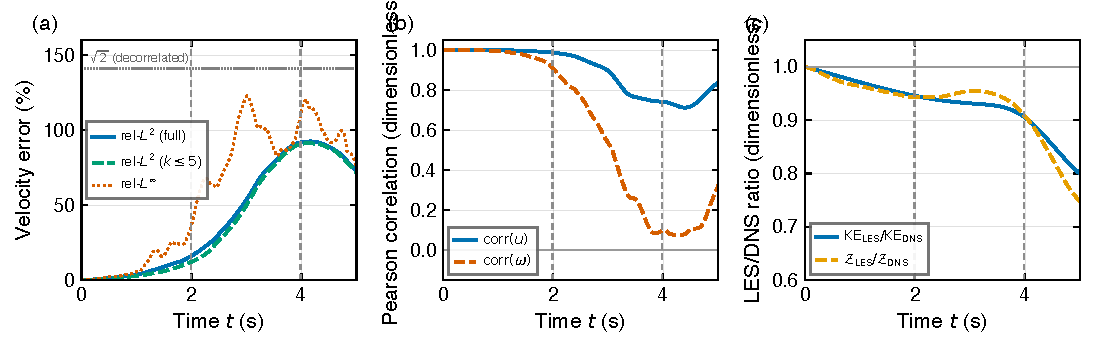
\includegraphics[width=\textwidth]{figures/results/les_sameic_predictability.pdf}
    \caption{Frame-by-frame comparison of a same-initial-condition reference LES against the DNS over $t\in[0,5]$~s ($Re=10^4$). (a) Velocity relative errors: full-field and resolved-band ($k\le 5$) relative-$L^2$, and relative-$L^\infty$ (\%); the grey dotted line marks the $\sqrt{2}$ fully-decorrelated level. (b) Pearson field correlations of velocity $u$ and vorticity $\omega$ (dimensionless). (c) LES/DNS ratios of kinetic energy and enstrophy $\mathcal{Z}=\langle\omega^2/2\rangle$ (dimensionless). Vertical dashed lines: one and two eddy-turnover times ($t_{\rm eddy}=1.99$~s).}
    \label{fig:les_predictability}
\end{figure}

\begin{figure}[!htbp]
    \centering
    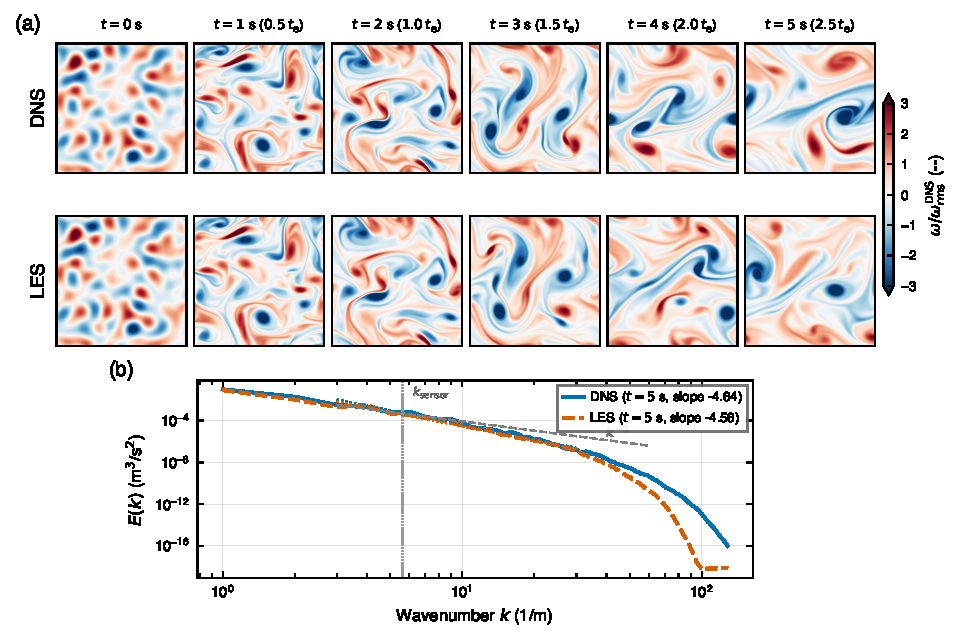
\includegraphics[width=\textwidth]{figures/results/dns_les_vorticity_compare.pdf}
    \caption{Same-initial-condition LES against the DNS ($Re=10^4$, periodic domain $[0,1]^2$~m). (a) Vorticity fields of the DNS (top) and the LES (bottom) at matched times $t\in\{0,1,2,3,4,5\}$~s; each time column is normalised by the DNS RMS vorticity, with colour showing $\omega/\omega_{\rm rms}^{\rm DNS}$ (dimensionless). (b) Radial energy spectrum $E(k)$ (m$^3$/s$^2$) of the LES and DNS at the matched final time $t=5$~s, with $k\in[3,30]$ slope fits and the $k^{-3}$ enstrophy-cascade reference; the vertical dotted line marks the $K=100$ sensor Nyquist $k_{\rm sensor}\approx 5.64$~m$^{-1}$. Eddy-turnover time $t_{\rm eddy}=1.99$~s.}
    \label{fig:les_vort_compare}
\end{figure}

\paragraph{Spectrum offset.}
Over the inertial range $k\in[3,30]$ the same-initial-condition LES and DNS energy spectra agree (slopes $-4.56$ and $-4.64$; Fig.~\ref{fig:les_vort_compare}b), while the LES energy falls below the DNS for $k\gtrsim 30$, where the hyperviscosity closure drains the small scales. This high-wavenumber offset bounds high-band reconstruction but not QR-pivot placement, which depends on the leading POD basis conditioning rather than the small-scale spectrum. The reference LES used for placement is integrated to $T_{\rm end}=50$ ($26.5\,t_{\rm eddy}$) for statistical convergence of the leading POD modes, since that convergence, not small-scale solver fidelity, governs the placement quality.

The LES-derived and DNS-oracle placements both target $K = 100$, with downstream KE MAPE within engineering tolerance (Table~\ref{tab:les_grid_independence}).

\begin{figure}[!htbp]
    \centering
    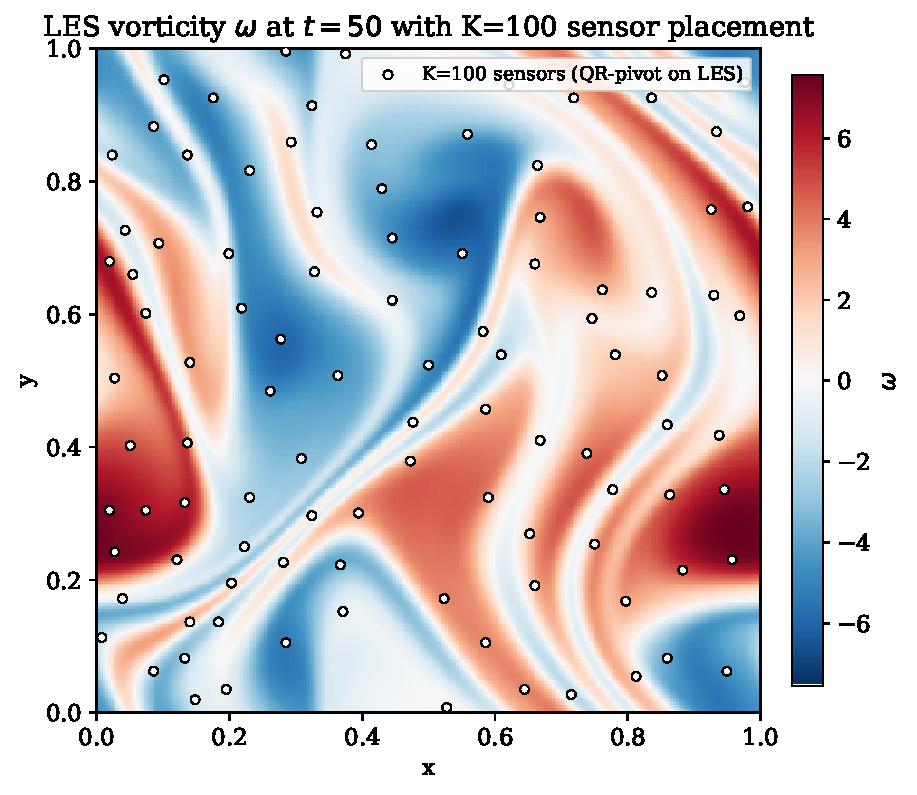
\includegraphics[width=0.7\linewidth]{figures/architecture/les_T50_vorticity_with_sensors.pdf}
    \caption{LES-derived sensor placement. Vorticity $\omega$ (1/s; $N_{\rm LES}=256$, $T_{\rm end}=50$) overlaid with $K=100$ QR-pivot sensor positions (markers) projected onto the DNS grid by nearest-neighbour mapping.}
    \label{fig:les_sensor_placement}
\end{figure}

\paragraph{Placement robustness to LES configuration.}
Grid independence in the DNS sense (Table~\ref{tab:dns_grid_indep}) does not transfer to the LES: the DNS converges to a resolved solution as $N$ increases, whereas an LES has no grid-converged limit short of DNS, since refining $N$ shifts the filter cutoff and the resolved/SGS split and thereby changes the resolved field itself. The relevant question is instead whether the \emph{placement} is robust to the LES configuration. The two LES runs compared (Table~\ref{tab:les_grid_independence}) differ not only in resolution ($N_{\rm LES}=256$ vs $128$) but also in closure (pure hyperviscosity vs Bardina-plus-hyperviscosity), hyperviscosity strength, and integration horizon ($T_{\rm end}=50$ vs $15$); despite this four-way change and a $16\times$ compute reduction, the downstream KE MAPE differs by only $0.04\%$ absolute ($\approx 0.3\%$ relative). The leading POD modes driving QR-pivot placement are therefore insensitive to the LES configuration, not merely to its resolution. The two retrainings here use a legacy single-seed, reduced-collocation configuration, so their absolute KE MAPE ($\approx 12\%$) sits above the final-protocol baseline; only the near-zero difference between them, the placement-robustness quantity, is used as evidence.

\begin{table}[!htbp]
    \centering
    \caption{LES configuration robustness: downstream KE MAPE after the full pipeline (LES POD basis $\to$ QR-pivot $\to$ sensor measurement $\to$ PI-CON retraining) under two LES runs that differ in resolution, closure, hyperviscosity strength, and integration horizon. The $E(k)$ slope is measured for $k>k_f$ (1/s units); the low-fidelity $-14$ reflects over-dissipation, and the $\approx 0.3\%$ relative difference lies at the evaluator noise floor. Both rows use a legacy single-seed, reduced-collocation retraining, so the absolute KE MAPE exceeds the final-protocol baseline; the placement-robustness claim rests on their relative difference, not the absolute level.}
    \label{tab:les_grid_independence}
    \footnotesize
    \setlength{\tabcolsep}{5pt}
    \begin{tabular}{lccccc}
    \toprule
    \textbf{Configuration} & \textbf{$N_{\rm LES}$} & \textbf{$T_{\rm end}$ (s)} & \textbf{Closure} & \textbf{$E(k)$ slope} & \textbf{KE MAPE} \\
    \midrule
    Reference LES    & $256^2$ & $50$ & hyperviscosity      & $-6.46$ & $12.36\%$ \\
    Low-fidelity LES & $128^2$ & $15$ & Bardina $+$ hyperv. & $-14$   & $12.40\%$ \\
    \midrule
    Difference       & --     & --  & --                 & --     & \textbf{$\approx 0.3\%$ rel.} \\
    \bottomrule
    \end{tabular}
\end{table}

\section{Sensor Data Construction}
\label{sec:sensor_data}

\paragraph{Pipeline alignment.}
For the LES-derived placement, data construction follows the deployment order: the LES determines where sensors are placed (positions only; the LES supplies no sensor values), and the physical flow determines what they measure. In this controlled study a DNS field stands in for the real-world flow, sampled at the $K$ sensor positions alone, so the model receives time-stamped $u,v$ values at fixed locations; the full DNS field is never read during training.

\paragraph{Sensor placement.}
The QRCP-on-POD-basis procedure of \S\ref{sec:sensor_placement} selects $K = 100$ grid indices and their physical coordinates from $\mathbf{X}\in\mathbb{R}^{N\times 201}$.

\paragraph{Sensor measurement values.}
Each sensor record contains time stamps and the corresponding $u,v$ velocities at the selected positions, with $N_t = 201$ aligned to the DNS frames. Vorticity is a derived diagnostic and pressure a model-internal variable; neither is used as supervision.

\paragraph{Normalization.}
Sensor values are standardized per channel,
\begin{equation}
    \hat{u}_{k,n} \;=\; \frac{u_{k,n} - \mu_u}{\sigma_u},\quad \hat{v}_{k,n} \;=\; \frac{v_{k,n} - \mu_v}{\sigma_v},
\end{equation}
where $\mu, \sigma$ are computed from all $K\cdot N_t$ measurements. The query-side prediction is inverse-transformed to recover the physical scale. The Reynolds number is normalized as $Re_{\text{norm}} = (Re - 5\,500) / 4\,000$, with offset and scale matching the approximate median and standard deviation of $\{100, 1\,000, 10\,000, 100\,000\}$ for multi-$Re$ training.

\paragraph{Train/validation split.}
At each step, an $80\%$ random subset of (time-index, space-index, channel-index) triples forms the training mini-batch; the remaining $20\%$ is held out as an in-sample interpolation check. The primary evaluation is the a posteriori field-reconstruction error against DNS (\S\ref{sec:eval_metrics}). Because the sensor (branch) input is identical for both subsets, this split monitors only transductive overfitting, memorising the specific space--time query coordinates seen in training; it is a sensor-consistency diagnostic and does not test generalisation to unseen sensor streams or flow conditions.

\section{Evaluation Metrics}
\label{sec:eval_metrics}

All metrics are computed post-training on a $128\times 128$ grid (the stored $256\times 256$ DNS snapshots are downsampled to $128^2$) so that finite-difference derivatives (divergence, vorticity) are evaluated below the stored-grid Nyquist wavenumber, where the central-difference stencil is uncontaminated by spectral-truncation noise near $k\to k_{\max}^{256}$.

\subsection{Field-Level Errors}

The error budget is reported at three levels: (i) a global, time-averaged $L_2$ norm; (ii) a pointwise worst-case ($L_\infty$) norm capturing localised peak error; (iii) a snapshot error at the final time $t^\star = T = 5$, the most demanding instant under the chaotic horizon (the trajectory spans $\approx 2.5$ eddy-turnover times). The definitions follow the PINN sparse-sensor reconstruction literature~\cite{Raissi2019JCP,Wang2024JMLR} and classical CFD validation practice~\cite{Pope2000}.

\paragraph{Relative $L_2$ error.}
For $\phi \in \{u, v, \omega, p\}$, following the normalised $L_2$ convention of~\cite{Raissi2019JCP},
\begin{equation}
    \mathrm{rel}\,L_2(\phi) \;=\; \frac{\Vert \phi_{\text{pred}} - \phi_{\text{DNS}}\Vert_2}{\Vert \phi_{\text{DNS}}\Vert_2},
\end{equation}
reported as a time-averaged value (mean over $t\in[0,T]$).

\paragraph{Relative $L_\infty$ (maximum) error.}
The worst-case pointwise discrepancy normalised by the maximum DNS amplitude,
\begin{equation}
    \label{eq:rel_linf}
    \mathrm{rel}\,L_\infty(\phi) \;=\; \frac{\max_{\mathbf{x},\,t}\,|\phi_{\text{pred}}(\mathbf{x},t) - \phi_{\text{DNS}}(\mathbf{x},t)|}{\max_{\mathbf{x},\,t}\,|\phi_{\text{DNS}}(\mathbf{x},t)|},
\end{equation}
captures localised peak discrepancies (e.g.\ unresolved shear-layer cusps) that the global $L_2$ averages out. The maximum runs over the $128^2$ grid and all $201$ time stamps.

\paragraph{Snapshot error at $t^\star = T$.}
The relative $L_2$ error of the final snapshot is reported separately, since forward integration accumulates phase error along the chaotic trajectory and $t^\star = 5$ is the most demanding instant:
\begin{equation}
    \label{eq:rel_l2_tstar}
    \mathrm{rel}\,L_2^{\,t^\star}(\phi) \;=\; \frac{\Vert \phi_{\text{pred}}(\cdot,\,t^\star) - \phi_{\text{DNS}}(\cdot,\,t^\star)\Vert_2}{\Vert \phi_{\text{DNS}}(\cdot,\,t^\star)\Vert_2}.
\end{equation}
A bounded snapshot error at $t^\star$ indicates the operator retains physical fidelity at the trajectory end, not only in time-averaged statistics.

\paragraph{Kinetic-energy MAPE.}
The integrated kinetic energy is the canonical CFD validation observable for turbulent statistics~\cite{Pope2000}. Its Mean Absolute Percentage Error (MAPE) is
\begin{equation}
    \mathrm{KE}(t) \;=\; \tfrac{1}{2}\int_\Omega \big(u^2 + v^2\big)\,d\mathbf{x},\qquad
    \mathrm{KE\_MAPE}(t) = \frac{|\mathrm{KE}_{\text{pred}}(t) - \mathrm{KE}_{\text{DNS}}(t)|}{\mathrm{KE}_{\text{DNS}}(t)}.
\end{equation}
The scalar reported in tables and figures is the time-mean $\overline{\mathrm{KE\_MAPE}} = \tfrac{1}{|T|}\sum_t \mathrm{KE\_MAPE}(t)$ over the evaluation window $t\in[0,5]$~s. This time-averaged relative error of $\mathrm{KE}(t)$ is the quantity referred to as the \emph{KE relative error} elsewhere in the text; the two names denote the same metric.

\paragraph{Enstrophy relative error.}
A second-order vorticity quantity with $\omega = \partial_x v - \partial_y u$:
\begin{equation}
    \mathrm{Ens}(t) \;=\; \tfrac{1}{2}\int_\Omega \omega^2\,d\mathbf{x},\qquad
    \mathrm{Ens\_rel\_err}(t) \;=\; \frac{|\mathrm{Ens}_{\text{pred}}(t) - \mathrm{Ens}_{\text{DNS}}(t)|}{\mathrm{Ens}_{\text{DNS}}(t)}.
\end{equation}

\subsection{Physics Consistency}

\paragraph{Divergence $L_2$.}
The incompressibility residual, evaluated on a finite-difference grid where the spectral-exact constraint $\nabla\!\cdot\!\mathbf{u} = 0$ is no longer at machine precision, is reported as both an absolute norm and a scale-normalised ratio. The ratio follows the dimensional-analysis convention of normalising solenoidal violations by the local strain-rate norm, enabling cross-resolution comparison~\cite{Pope2000,Moin1998AIAA}:
\begin{equation}
    \mathrm{div}\_L_2(t) \;=\; \big\Vert \partial_x u_{\text{pred}} + \partial_y v_{\text{pred}} \big\Vert_2.
\end{equation}
The spectral DNS is divergence-free in spectral space but not in finite-difference space, giving an evaluation-grid floor $\Vert\nabla\cdot\mathbf{u}\Vert_2 \approx 0.092$ ($1.04\%$ of the DNS strain rate $\Vert\nabla\mathbf{u}\Vert_F^{\rm DNS}$; Table~\ref{tab:dns_verification}). This floor is the truncation error of the second-order central-difference operator on the $128^2$ evaluation grid and scales with the resolved high-wavenumber content: spectrally low-pass filtering the DNS reference to $k\le 16$ lowers it to $0.38\%$, and to $k\le 5$ to $0.07\%$. The floor is therefore a property of the field's bandwidth under the chosen operator, not an absolute incompressibility limit; a reconstruction confined to low wavenumbers is expected to register a smaller value for this reason alone. The relative divergence ratio
\begin{equation}
    \mathrm{div}\_\mathrm{ratio} \;=\; \Vert\nabla\cdot\mathbf{u}_{\rm pred}\Vert_2 \big/ \Vert\nabla\mathbf{u}\Vert_F^{\rm DNS}
\end{equation}
places model values on the same scale, with $\Vert\nabla\mathbf{u}\Vert_F^{\rm DNS} = 8.898$ on the evaluation grid (\S\ref{subsec:dns_verification}).

\paragraph{NS residual r.m.s.}
The root-mean-square of the NS momentum and continuity residuals at $N_c$ collocation points,
\begin{equation}
    \label{eq:ns_rms}
    \mathrm{NS\_rms}_\phi \;=\; \sqrt{\frac{1}{N_c}\sum_{j=1}^{N_c} \mathcal{R}_\phi^2(\mathbf{x}_j,t_j)}, \quad \phi \in \{u,\, v,\, c\},
\end{equation}
with $\mathcal{R}_u$, $\mathcal{R}_v$, $\mathcal{R}_c$ defined in \eqref{eq:res_u}--\eqref{eq:cont_res}. The continuity variant is also written $\mathrm{div\_rms}$. Values are compared against the DNS reference computed on the downsampled grid.

\subsection{Spectral Diagnostics}

\paragraph{Per-band relative error.}
The KE spectrum is grouped along the K=100 sensor Nyquist cutoff $k_{\max}^{\rm sensor} = \lfloor \sqrt{K/\pi} \rfloor = \lfloor 5.64 \rfloor = 5$ (the integer band edge; the unfloored $\sqrt{K/\pi}\approx 5.64$ appears in the spectral plots). This cutoff is the two-dimensional Nyquist wavenumber for $K$ samples over a unit-area domain (one sample per $\pi/K$ wavenumber cell), the spatial-sampling analogue of the one-dimensional Nyquist limit; above it the $K$ sensors cannot constrain independent Fourier modes. The bands are: a low band ($k \le 5$, below the sensor Nyquist cutoff $k_{\max}^{\rm sensor}\approx 5.64$, which carries $\approx 99\%$ of the total energy at $t=5$, and $\approx 95\%$ time-averaged over $t\in[0,5]$, the lower mean reflecting the broadband initial condition during spin-up; fully sensor-resolvable), a mid band ($5 < k \le 16$, transitional), and a high band ($k > 16$, above the sensor Nyquist cutoff). For each band,
\begin{equation}
    \mathrm{band\_rel\_err}(t) \;=\; \frac{|E_{\text{band, pred}}(t) - E_{\text{band, DNS}}(t)|}{E_{\text{band, DNS}}(t)}.
\end{equation}

\paragraph{Forcing-mode amplitude and phase.}
Since $k_f = 2$ carries the sustained energy injection, its reconstruction is reported separately. From the Fourier coefficient $\hat{u}_{k_f}$,
\begin{equation}
    \mathrm{amp\_ratio}(t) \;=\; \frac{|\hat{u}^{\text{pred}}_{k_f}|}{|\hat{u}^{\text{DNS}}_{k_f}|},\quad
    \mathrm{phase\_err}(t) \;=\; \arg(\hat{u}^{\text{pred}}_{k_f}) - \arg(\hat{u}^{\text{DNS}}_{k_f}).
\end{equation}
The ideal values are $\mathrm{amp\_ratio} = 1$ and $\mathrm{phase\_err} = 0$.

\paragraph{Time-segment decomposition.}
Metrics are also reported as means over three segments: early ($t<1$), mid ($1\le t<3$), late ($t\ge 3$).

\paragraph{Wavelet-based multi-scale error diagnostic.}
Complementing the Fourier-band diagnostics, a 2D Daubechies-4 wavelet decomposition is applied to the reconstructed field. The wavelet metric decomposes the relative $L_2$ error by level, providing the spatial localisation that the global Fourier spectrum lacks. Full details are in Appendix~\ref{app:wavelet_diag}.

\subsection{Train/Validation Split Metrics}
To detect transductive overfitting, KE MAPE is reported over the training window $t\in[0, 4]$ and the validation window $t\in[4, 5]$ separately.

\section{Ablation and Reference Comparisons}
\label{sec:baselines}

The final result set contextualises PI-CON through matched architecture ablations and reference-only diagnostics. The classical-interpolation baselines (RBF, IDW, and divergence-free trigonometric least squares) are regenerated on the final LES-derived placement and reported in Appendix~\ref{app:fair_baselines}; older Standard-PINN development comparisons are not used as thesis evidence because they were not regenerated under the final $20\,000$-iteration, $1024$-collocation PI-CON protocol.

\paragraph{Matched architecture ablations.}
The four neural variants reconstruct the field from the same $K=100$ sensor stream as PI-CON and require no DNS full-field access at training or inference:
\begin{itemize}
    \item \textbf{Vanilla DeepONet} (B0): the same operator backbone without CfC temporal encoding and without cross-attention; the architectural reference for the $2\times2$ ablation matrix.
    \item \textbf{CfC-only} (B1): B0 plus CfC temporal encoding, but without cross-attention.
    \item \textbf{Cross-attention-only} (B2): B0 plus query-conditional cross-attention, but without CfC temporal encoding.
    \item \textbf{Full PI-CON} (B3): CfC temporal encoding and query-conditional cross-attention together.
\end{itemize}

\paragraph{Reference-only baseline (not engineering-transferable).}
\textbf{Gappy POD} requires the full DNS snapshot matrix to build its POD basis and is \emph{not engineering-transferable} under the deployment regime of \S\ref{sec:engineering_constraint}; it is reported only as an upper reference for spectral-truncation reconstruction quality, not as a comparable method. The \textbf{forward-CFD initial-condition reconstruction} likewise needs offline DNS snapshots for its POD basis and is labelled accordingly.

\section{Open-Source Availability}
\label{sec:impl_env}

The implementation is available at \url{https://github.com/latteine1217/pi-lnn}. Statistical comparisons use five independent seeds with Welch's two-sample $t$-test and Cohen's $d$ effect size.
